\ifdraft TODO

\chapter{The TCP Models}
\label{cha:tcp}

\section{The TCP Module}

The \nedtype{Tcp} model relies on sending and receiving \cppclass{IPControlInfo} objects
attached to TCP segment objects as control info (see \ffunc{cMessage::setControlInfo()}).

The \nedtype{Tcp} module manages several \cppclass{TcpConnection} object each
holding the state of one connection. The connections are identified
by a connection identifier which is choosen by the application.
If the connection is established it can also be identified by
the local and remote addresses and ports. The TCP module simply
dispatches the incoming application commands and packets to
the corresponding object.

\subsection{TCP packets}
\label{subsec:tcp_packets}

The INET framework models the TCP header with the \msgtype{TcpHeader} message class.
This contains the fields of a TCP frame, except:
\begin{compactitem}
  \item \emph{Data Offset}: represented by \ffunc{cMessage::length()}
  \item \emph{Reserved}
  \item \emph{Checksum}: modelled by \ffunc{cMessage::hasBitError()}
  \item \emph{Options}: only EOL, NOP, MSS, WS, SACK\_PERMITTED, SACK and TS are possible
  \item \emph{Padding}
\end{compactitem}

The Data field can either be represented by (see \cppclass{TcpDataTransferMode}):
\begin{compactitem}
  \item encapsulated C++ packet objects,
  \item raw bytes as a \cppclass{ByteArray} instance,
  \item its byte count only,
\end{compactitem}
corresponding to transfer modes OBJECT, BYTESTREAM, BYTECOUNT resp.


\subsection{TCP commands}

The application and the TCP module communicates with each other
by sending \cppclass{cMessage} objects. These messages are specified
in the \ffilename{TCPCommand.msg} file.

The \cppclass{TCPCommandCode} enumeration defines the message kinds
that are sent by the application to the TCP:
\begin{itemize}
  \item TCP\_C\_OPEN\_ACTIVE: active open
  \item TCP\_C\_OPEN\_PASSIVE: passive open
  \item TCP\_C\_SEND: send data
  \item TCP\_C\_CLOSE: no more data to send
  \item TCP\_C\_ABORT: abort connection
  \item TCP\_C\_STATUS: request status info from TCP
\end{itemize}

Each command message should have an attached control info of type \cppclass{TcpCommand}.
Some commands (TCP\_C\_OPEN\_xxx, TCP\_C\_SEND) use subclasses.
The \cppclass{TcpCommand} object has a \fvar{connId} field that identifies the
connection locally within the application. \fvar{connId} is to be chosen by the
application in the open command.

When the application receives a message from the TCP, the message kind is
set to one of the \cppclass{TCPStatusInd} values:
\begin{itemize}
  \item TCP\_I\_ESTABLISHED: connection established
  \item TCP\_I\_CONNECTION\_REFUSED: connection refused
  \item TCP\_I\_CONNECTION\_RESET: connection reset
  \item TCP\_I\_TIME\_OUT: connection establish timer went off, or max retransmission count reached
  \item TCP\_I\_DATA: data packet
  \item TCP\_I\_URGENT\_DATA: urgent data packet
  \item TCP\_I\_PEER\_CLOSED: FIN received from remote TCP
  \item TCP\_I\_CLOSED: connection closed normally
  \item TCP\_I\_STATUS: status info
\end{itemize}

These messages also have an attached control info with \cppclass{TcpCommand}
or derived type (TCPConnectInfo, TCPStatusInfo, TCPErrorInfo).

% receive() calls are not modeled, incoming data passed to the application right away
% how accurate the modeling of the receiver window?

\subsection{TCP parameters}

The \nedtype{Tcp} module has the following parameters:
\begin{itemize}
  \item \fpar{advertisedWindow} in bytes, corresponds with the maximal receiver buffer capacity (Note: normally, NIC queues should be at least this size, default is  14*mss)
  \item \fpar{delayedAcksEnabled} delayed ACK algorithm (RFC 1122) enabled/disabled
  \item \fpar{nagleEnabled} Nagle's algorithm (RFC 896) enabled/disabled
  \item \fpar{limitedTransmitEnabled} Limited Transmit algorithm (RFC 3042) enabled/disabled (can be used for TCPReno/TCPTahoe/TCPNewReno/TCPNoCongestionControl)
  \item \fpar{increasedIWEnabled} Increased Initial Window (RFC 3390) enabled/disabled
  \item \fpar{sackSupport} Selective Acknowledgment (RFC 2018, 2883, 3517) support (header option) (SACK will be enabled for a connection if both endpoints support it)
  \item \fpar{windowScalingSupport} Window Scale (RFC 1323) support (header option) (WS will be enabled for a connection if both endpoints support it)
  \item \fpar{timestampSupport} Timestamps (RFC 1323) support (header option) (TS will be enabled for a connection if both endpoints support it)
  \item \fpar{mss} Maximum Segment Size (RFC 793) (header option, default is 536)
  \item \fpar{tcpAlgorithmClass} the name of TCP flavour

             Possible values are ``TCPReno'' (default), ``TCPNewReno'', ``TCPTahoe'', ``TCPNoCongestionControl'' and ``DumpTCP''.
             In the future, other classes can be written which implement Vegas, LinuxTCP  or other variants.
             See section \ref{sec:tcp_algorithms} for detailed description of implemented flavours.

             Note that TCPOpenCommand allows tcpAlgorithmClass to be chosen per-connection.

  \item \fpar{recordStats} if set to false it disables writing excessive amount of output vectors
\end{itemize}

\section{TCP connections}

Most part of the TCP specification is implemented in the
\cppclass{TcpConnection} class: takes care of the state machine,
stores the state variables (TCB), sends/receives SYN, FIN, RST, ACKs, etc.
TCPConnection itself implements the basic TCP ``machinery'',
the details of congestion control are factored out to
\cppclass{TcpAlgorithm} classes.

There are two additional objects the \cppclass{TcpConnection}
relies on internally: instances of \cppclass{TcpSendQueue} and
\cppclass{TcpReceiveQueue}. These polymorph classes manage the actual data stream,
so \cppclass{TcpConnection} itself only works with sequence number variables.
This makes it possible to easily accomodate need for various types of
simulated data transfer: real byte stream, "virtual" bytes (byte counts
only), and sequence of \cppclass{cMessage} objects (where every message object is
mapped to a TCP sequence number range).

\subsection{Data transfer modes}

Different applications have different needs how to represent
the messages they communicate with. Sometimes it is enough to
simulate the amount of data transmitted (``200 MB''), contents
does not matter. In other scenarios contents matters a lot.
The messages can be represented as a stream of bytes, but
sometimes it is easier for the applications to pass message
objects to each other (e.g. HTTP request represented by a
\msgtype{HTTPRequest} message class).

The TCP modules in the INET framework support 3 data transfer modes:

\begin{itemize}
  \item \ttt{TCP\_TRANSFER\_BYTECOUNT}: only byte counts are
        represented, no actual payload in \msgtype{TcpHeader}s.
        The TCP sends as many TCP segments as needed
  \item \ttt{TCP\_TRANSFER\_BYTESTREAM}: the application can pass
        byte arrays to the TCP. The sending TCP breaks down the bytes
        into MSS sized chunks and transmits them as the payload
        of the TCP segments. The receiving application can read the
        chunks of the data.
  \item \ttt{TCP\_TRANSFER\_OBJECT}: the application pass a
        \cppclass{cMessage} object to the TCP. The sending
        TCP sends as many TCP segments as needed according to
        the message length. The \cppclass{cMessage} object
        is also passed as the payload of the first segment. % check: first?
        The receiving application receives the object only
        when its last byte is received.
\end{itemize}

These values are defined in \ffilename{TCPCommand.msg} as
the \cppclass{TcpDataTransferMode} enumeration. The application
can set the data transfer mode per connection when the connection
is opened. The client and the server application must specify
the same data transfer mode.


\subsection{Opening connections}

Applications can open a local port for incoming connections by sending
the TCP a TCP\_C\_PASSIVE\_OPEN message. The attached control info
(an \cppclass{TcpOpenCommand}) contains the local address and port.
The application can specify that it wants to handle
only one connection at a time, or multiple simultanous connections. If the
\fvar{fork} field is true, it emulates the Unix accept(2) semantics: a new
connection structure is created for the connection (with a new \fvar{connId}),
and the connection with the old connection id remains listening.
If \fvar{fork} is false, then the first connection is accepted
(with the original \fvar{connId}),
and further incoming connections will be refused by the TCP by sending an RST segment.
The \fvar{dataTransferMode} field in \cppclass{TcpOpenCommand} specifies
whether the application data is transmitted as C++ objects, real bytes or byte
counts only. The congestion control algorithm can also be specified
on a per connection basis by setting \fvar{tcpAlgorithmClass} field to the
name of the algorithm.

The application opens a connection to a remote server by sending the TCP
a TCP\_C\_OPEN\_ACTIVE command. The TCP creates a \cppclass{TcpConnection}
object an sends a SYN segment. The initial sequence number selected according
to the simulation time: 0 at time 0, and increased by 1 in each 4$\mu$s.
If there is no response to the SYN segment, it retry after 3s, 9s, 21s and
45s. After 75s a connection establishment timeout (TCP\_I\_TIMEOUT) reported
to the application and the connection is closed.

When the connection gets established, TCP sends a TCP\_I\_ESTABLISHED
notification to the application. The attached control info
(a \cppclass{TcpConnectInfo} instance)
will contain the local and remote addresses and ports of the connection.
If the connection is refused by the remote peer (e.g. the port is not open),
then the application receives a TCP\_I\_CONNECTION\_REFUSED message.

\begin{note}
If you do active OPEN, then send data and close before the connection
has reached ESTABLISHED, the connection will go from SYN\_SENT to CLOSED
without actually sending the buffered data. This is consistent with
RFC 793 but may not be what you would expect.
\end{note}

\begin{note}
Handling segments with SYN+FIN bits set (esp. with data too) is
inconsistent across TCPs, so check this one if it is of importance.
\end{note}

\subsection{Sending Data}

The application can write data into the connection
by sending a message with TCP\_C\_SEND kind to the TCP.
The attached control info must be of type \cppclass{TCPSendCommand}.

The TCP will add the message to the \emph{send queue}.
There are three type of send queues corresponding to the
three data transfer mode. If the payload is transmitted as a message
object, then \cppclass{TCPMsgBasedSendQueue};
if the payload is a byte array then \cppclass{TCPDataStreamSendQueue};
if only the message lengths are represented then \cppclass{TCPVirtualDataSendQueue}
are the classes of send queues. The appropriate queue is created based
on the value of the \fpar{dataTransferMode} parameter of the Open command, no
further configuration is needed.

The message is handed over to the IP when there is
enough room in the windows. If Nagle's algorithm is
enabled, the TCP will collect 1 SMSS data and sends
them toghether.

\begin{note}
There is no way to set the PUSH and URGENT flags, when sending data.
\end{note}

% FIXME urgBit is never set
% FIXME model TCP_NODELAY, there is no PUSH flag in socket.send() (TCP_PUSH option ?)

\subsection{Receiving Data}

The TCP connection stores the incoming segments in the
\emph{receive queue}. The receive queue also has three flavours:
\cppclass{TCPMsgBasedRcvQueue}, \cppclass{TCPDataStreamRcvQueue}
and \cppclass{TCPVirtualDataRcvQueue}. The queue is created
when the connection is opened according to the \fvar{dataTransferMode}
of the connection.

Finite receive buffer size is modeled by the \fpar{advertisedWindow}
parameter. If receive buffer is exhausted (by out-of-order
segments) and the payload length of a new received segment
is higher than the free receiver buffer, the new segment will be dropped.
Such drops are recorded in \emph{tcpRcvQueueDrops} vector.

If the \emph{Sequence Number} of the received segment is the next
expected one, then the data is passed
to the application immediately. The \ffunc{recv()} call of
Unix is not modeled.

The data of the segment, which can be either a \cppclass{cMessage}
object, a \cppclass{ByteArray} object, or a simply byte count,
is passed to the application in a message that has
TCP\_I\_DATA kind.

% when the cMessage object is passed to the app? when last byte received?

\begin{note}
The TCP module does not handle the segments with PUSH or URGENT
flags specially. The data of the segment passed to the application
as soon as possible, but the application can not find out if that
data is urgent or pushed.
\end{note}

\subsection{RESET handling}

When an error occures at the TCP level, an RST segment is sent to
the communication partner and the connection is aborted.
Such error can be:
\begin{compactitem}
  \item arrival of a segment in CLOSED state
  \item an incoming segment acknowledges something not yet sent.
\end{compactitem}

The receiver of the RST it will abort the connection.
If the connection is not yet established, then the passive
end will go back to the LISTEN state and waits for another
incoming connection instead of aborting.

\subsection{Closing connections}

When the application does not have more data to send, it closes the
connection by sending a TCP\_C\_CLOSE command to the TCP. The TCP
will transmit all data from its buffer and in the last segment sets
the FIN flag. If the FIN is not acknowledged in time it will be
retransmitted with exponential backoff.

The TCP receiving a FIN segment will notify the application that
there is no more data from the communication partner. It sends
a TCP\_I\_PEER\_CLOSED message to the application containing
the connection identifier in the control info.

When both parties have closed the connection, the applications
receive a TCP\_I\_CLOSED message and the connection object is
deleted. (Actually one of the TCPs waits for $2 MSL$ before
deleting the connection, so it is not possible to reconnect
with the same addresses and port numbers immediately.)

\subsection{Aborting connections}

The application can also abort the connection. This means that
it does not wait for incoming data, but drops the data associated
with the connection immediately. For this purpose the application
sends a TCP\_C\_ABORT message specifying the connection identifier
in the attached control info. The TCP will send a RST to the
communication partner and deletes the connection object. The application
should not reconnect with the same local and remote addresses and
ports within MSL (maximum segment lifetime), because segments
from the old connection might be accepted in the new one.

\subsection{Status Requests}

Applications can get detailed status information about an existing
connection. For this purpose they send the TCP module a TCP\_C\_STATUS
message attaching an \cppclass{TcpCommand} info with the identifier
of the connection. The TCP will respond with a TCP\_I\_STATUS message
with a \cppclass{TcpStatusInfo} attachement. This control info
contains the current state, local and remote addresses and ports,
the initial sequence numbers, windows of the receiver and sender, etc.

% \section{TCP queues}
%
% Three queues belong to each TCP connection. The \emph{send queue} holds
% the segments not yet transmitted or not yet acknowledged.
% The \emph{receive queue} holds the segments received by the TCP,
% but not yet passed to the application. (This happens only when the segment
% is received out-of-order.). The \emph{retransmit queue} holds additional
% information about the segments in the send queue.
%
% As mentioned in section \ref{subsec:tcp_packets}, there are three methods
% to represent the application data in the TCP segment. Consequently the above
% queues comes in three flavours. If the payload is transmitted as a message
% object, then \cppclass{TCPMsgBasedRcvQueue} and \cppclass{TCPMsgBasedSendQueue};
% if the payload is a byte array then \cppclass{TCPDataStreamRcvQueue} and
% \cppclass{TCPDataStreamSendQueue}; if only the message lengths are represented
% then \cppclass{TCPVirtualDataRcvQueue} and \cppclass{TCPVirtualDataSendQueue}
% are the classes of receive/send queues. The appropriate queue is created based
% on the value of the \fpar{dataTransferMode} parameter of the Open command, no
% further configuration is needed. The retransmit queue is always an
% instance of \cppclass{TcpSackRexmitQueue}.
%
% The interfaces of the receive/send queues are defined by the
% \cppclass{TcpReceiveQueue} and \cppclass{TcpSendQueue} classes.
%
% % mapping segments into the sequence space
%

\section{TCP algorithms}
\label{sec:tcp_algorithms}

The \cppclass{TcpAlgorithm} object controls
retransmissions, congestion control and ACK sending: delayed acks, slow start,
fast retransmit, etc. They are all extends the \cppclass{TcpAlgorithm} class.
This simplifies the design of \cppclass{TcpConnection} and makes it a lot easier to
implement TCP variations such as Tahoe, NewReno, Vegas or LinuxTCP.

Currently implemented algorithm classes are \cppclass{TcpReno},
\cppclass{TcpTahoe}, \cppclass{TcpNewReno}, \cppclass{TcpNoCongestionControl}
and \cppclass{DumbTcp}. It is also possible to add new TCP variations
by implementing \cppclass{TcpAlgorithm}.

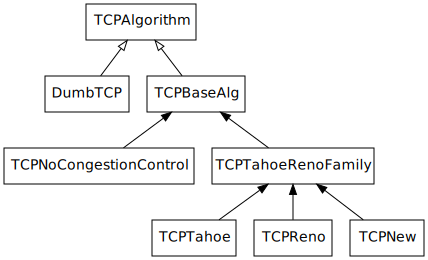
\includegraphics{figures/tcp_algorithms}

The concrete TCP algorithm class to use can be chosen per connection (in OPEN)
or in a module parameter.

\subsection{DumbTcp}

A very-very basic \cppclass{TcpAlgorithm} implementation, with hardcoded
retransmission timeout (2 seconds) and no other sophistication. It can be
used to demonstrate what happened if there was no adaptive
timeout calculation, delayed acks, silly window avoidance,
congestion control, etc. Because this algorithm does not
send duplicate ACKs when receives out-of-order segments,
it does not work well together with other algorithms.

\subsection{TcpBaseAlg}

The \cppclass{TcpBaseAlg} is the base class of the INET implementation
of Tahoe, Reno and New Reno. It implements basic TCP
algorithms for adaptive retransmissions, persistence timers,
delayed ACKs, Nagle's algorithm, Increased Initial Window
-- EXCLUDING congestion control. Congestion control
is implemented in subclasses.

\subsubsection*{Delayed ACK}

When the \fpar{delayedAcksEnabled} parameter is set to \fkeyword{true},
\cppclass{TcpBaseAlg} applies a 200ms delay before sending ACKs.

\subsubsection*{Nagle's algorithm}

When the \fpar{nagleEnabled} parameter is \fkeyword{true}, then
the algorithm does not send small segments if there is outstanding
data. See also \ref{subsec:trans_policies}.

\subsubsection*{Persistence Timer}

The algorithm implements \emph{Persistence Timer} (see \ref{subsec:flow_control}).
When a zero-sized window is received it starts the timer with 5s timeout.
If the timer expires before the window is increased, a 1-byte probe is
sent. Further probes are sent after 5, 6, 12, 24, 48, 60, 60, 60, ...
seconds until the window becomes positive.

\subsubsection*{Initial Congestion Window}

Congestion window is set to 1 SMSS when the connection is established.
If the \fpar{increasedIWEnabled} parameter is true, then the initial
window is increased to 4380 bytes, but at least 2 SMSS and at most 4 SMSS.
The congestion window is not updated afterwards; subclasses can
add congestion control by redefining virtual methods of the
\cppclass{TcpBaseAlg} class.

\subsubsection*{Duplicate ACKs}

The algorithm sends a duplicate ACK when an out-of-order
segment is received or when the incoming segment fills in all
or part of a gap in the sequence space.

\subsubsection*{RTO calculation}

Retransmission timeout ($RTO$) is calculated according to
Jacobson algorithm (with $\alpha=7/8$), and Karn's modification is also applied.
The initial value of the $RTO$ is 3s, its minimum is 1s,
maximum is 240s (2 MSL).

% FIXME according to RFC1222, MIN_REXMIT_TIMEOUT should be a fraction of second
%       to accomodate high speed LANs. In the linux kernel (net/tcp.h)
%       TCP_RTO_MIN is HZ/5 = 200ms. Consider 0ms lower bound.

\subsection{TCPNoCongestion}

TCP with no congestion control (i.e. congestion window kept very large).
Can be used to demonstrate effect of lack of congestion control.

% FIXME 65536 is not 'very large' nowadays, with window scaling
%       the receive window can be as large as 2^30 bytes.
%       Consequently the initial ssthresh is too small for Tahoe/Reno/NewReno,
%       Slow Start is stopped too early first time.

\subsection{TcpTahoe}

The \cppclass{TcpTahoe} algorithm class extends \cppclass{TcpBaseAlg}
with \emph{Slow Start}, \emph{Congestion Avoidance} and
\emph{Fast Retransmit} congestion control algorithms.
This algorithm initiates a \emph{Slow Start} when a packet
loss is detected.

\subsubsection*{Slow Start}

The congestion window is initially set to 1 SMSS or in case of
\fpar{increasedIWEnabled} is \fkeyword{true} to 4380 bytes
(but no less than 2 SMSS and no more than 4 SMSS). The window
is increased on each incoming ACK by 1 SMSS, so it is approximately
doubled in each RTT.

\subsubsection*{Congestion Avoidance}

When the congestion window exceeded $ssthresh$, the window
is increased by $SMSS^2/cwnd$ on each incoming ACK event, so
it is approximately increased by 1 SMSS per RTT.

\subsubsection*{Fast Retransmit}

When the 3rd duplicate ACK received, a packet loss is detected
and the packet is retransmitted immediately. Simultanously
the $ssthresh$ variable is set to half of the $cwnd$ (but at least 2 SMSS)
and $cwnd$ is set to 1 SMSS, so it enters slow start again.

Retransmission timeouts are handled the same way:
$ssthresh$ will be $cwnd/2$, $cwnd$ will be 1 SMSS.

\subsection{TcpReno}

The \cppclass{TcpReno} algorithm extends the behaviour \cppclass{TcpTahoe}
with \emph{Fast Recovery}. This algorithm can also use the information
transmitted in SACK options, which enables a much more accurate
congestion control.

\subsubsection*{Fast Recovery}

When a packet loss is detected by receiveing 3 duplicate ACKs,
$ssthresh$ set to half of the current window as in Tahoe. However
$cwnd$ is set to $ssthresh + 3*SMSS$ so it remains in congestion
avoidance mode. Then it will send one new segment for each incoming
duplicate ACK trying to keep the pipe full of data. This requires
the congestion window to be inflated on each incoming duplicate
ACK; it will be deflated to $ssthresh$ when new data gets
acknowledged.

However a hard packet loss (i.e. RTO events) cause a
slow start by setting $cwnd$ to 1 SMSS.

\subsubsection*{SACK congestion control}

This algorithm can be used with the SACK extension.
Set the \fpar{sackSupport} parameter to \fkeyword{true} to
enable sending and receiving \emph{SACK} options.

\subsection{TcpNewReno}

This class implements the TCP variant known as New Reno.
New Reno recovers more efficiently from multiple packet losses within one RTT
than Reno does.

It does not exit fast-recovery phase until all data which was out-standing
at the time it entered fast-recovery is acknowledged. Thus avoids
reducing the $cwnd$ multiple times.

\fi


